\documentclass[tikz]{standalone}
\usepackage{tikz}
\usetikzlibrary{positioning}


\begin{document}

\newcommand{\cost}{c}
\newcommand{\lightred}{white!60!red}
\newcommand{\partfrac}[2]{\frac{\partial #1}{\partial #2}}
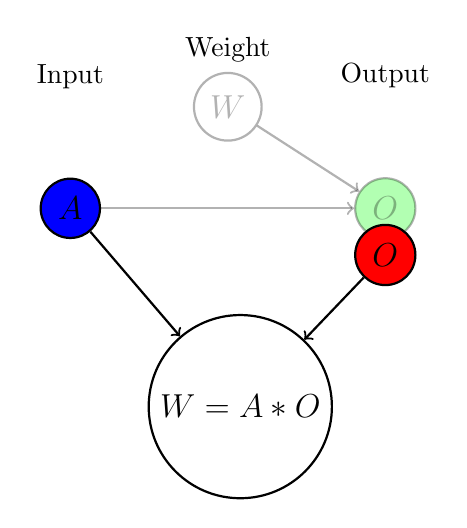
\begin{tikzpicture}[auto, node distance=4cm, every loop/.style={},
thick,main node/.style={circle,draw,font=\sffamily\large\bfseries}]

\node[main node] [fill=blue] [label={[shift={(0,1.0)}]Input}]  (A) {$A$};
\node[main node] [fill=green,opacity=0.3] [right of=A] [label={[shift={(0,1.0)}]Output}] (B) {$O$};
\node[main node] [] [below right = 1.41cm and 1.05cm of A] (C) {$\partfrac{W}{\cost} = A*\partfrac{O}{\cost}$};
\node[main node] [fill=red] (D)  [below = -0.2cm of B] {$\partfrac{O}{\cost}$};
\node[main node] [opacity=0.3] (E) [above right = 0.7cm and 1.41cm of A] [label={[shift={(0,0.0)}]Weight}]  {$W$};

\path[every node/.style={font=\sffamily\normalsize},opacity=0.3]
(A) [->] edge node {} (B)
(E) [->] edge node {} (B);
\path[every node/.style={font=\sffamily\normalsize}]
(D) [->] edge node [] {} (C)
(A) [->] edge node [] {} (C);
\end{tikzpicture}


\end{document}